\documentclass{article}
\PassOptionsToPackage{numbers,compress}{natbib}
\usepackage[preprint]{neurips_2025}
\makeatletter
\renewcommand{\@noticestring}{ECE 4424}
\makeatother

\usepackage[utf8]{inputenc}
\usepackage[T1]{fontenc}
\usepackage{hyperref}
\usepackage{url}
\usepackage{booktabs}
\usepackage{amsmath}
\usepackage{graphicx}
\usepackage{xcolor}
\usepackage{float}

\setlength{\textfloatsep}{8pt plus 2pt minus 2pt}
\setlength{\intextsep}{6pt plus 2pt minus 2pt}
\setlength{\floatsep}{6pt plus 2pt minus 2pt}
\newcommand{\todo}[1]{\textcolor{red}{[TODO: #1]}}

\title{Milestone Report: Using Synthetic Data for Automatic Gear Defect Detection}

\author{Haoxuan Yang (Individual)\\
Electrical Engineering}

\begin{document}
\maketitle

\section{Introduction}

Small impact damage on gear teeth, roughly 0.1--0.2\,mm across, is hard to see. LISA (Laser Inspection via Scattering Analysis) lights one tooth at a time with a laser line while the gear turns and flags teeth whose reflection looks abnormal for technician review. With only three physical gears available, real damaged examples are scarce, so we ask whether simulated laser-reflection data can make up for them. Synthetic images have helped defect segmentation on complex metal surfaces~\cite{fulir2023}. The simulation experiments in Mitsuba~3~\cite{mitsuba3} are done. The physical setup is under construction (Section~\ref{sec:apparatus}); its capture software is not written yet, so no real scans exist.

\textbf{Thesis.} For gear tooth inspection, we will test whether adding simulated laser-line reflection data to limited real scans helps detect impact damage for technician review, using real scans alone as the baseline and evaluating both approaches on a separate physical gear at steady and changing rotation speeds.

\textbf{Revisions since the proposal.} As the proposal feedback asked, the features and model are now specified (Section~\ref{sec:method}). The real-only against real-plus-synthetic comparison waits for real scans; here, simulated damage serves as validation and test data.

\section{Method}
\label{sec:method}

\subsection{Physical apparatus}
\label{sec:apparatus}

A $6.7\times0.1$\,mm, 650\,nm laser line hits one tooth from 300\,mm (Fig.~\ref{fig:setup}, left). A smooth tooth surface reflects the line mostly in one direction. A dent tilts small patches of the surface, so part of the light leaves at other angles. A 50\,mm plano-convex collector lens 25\,mm from the tooth turns each reflected ray's angle into a position on a translucent screen placed at its focal plane: position $=50\,\text{mm}\times\tan(\text{angle})$ in each screen direction. The screen image is therefore the angular distribution of the reflected light, and light scattered by a dent lands away from the main bright spot. A camera photographs the screen. A motor turns the gear through a 4:1 belt reduction, and a second belt drives a 600-pulse encoder at motor speed that will trigger the camera every 5 encoder counts, which is every $0.1875^\circ$ of gear rotation (Fig.~\ref{fig:setup}, right).

\begin{figure}[h]
  \centering
  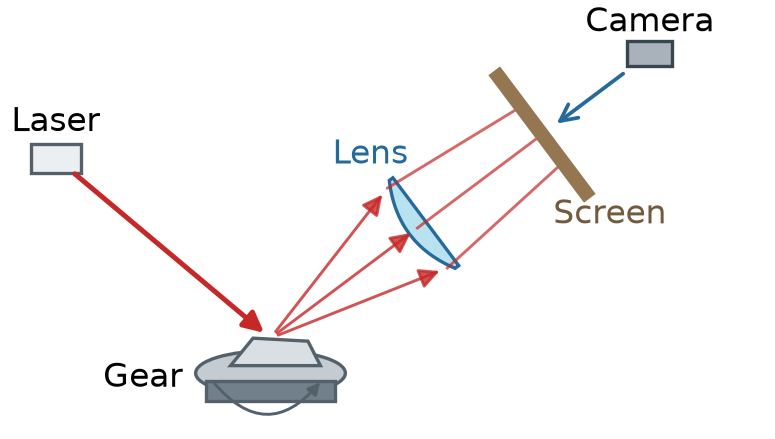
\includegraphics[height=2.7cm]{figures/setup_schematic_report.png}\hspace{1.5em}
  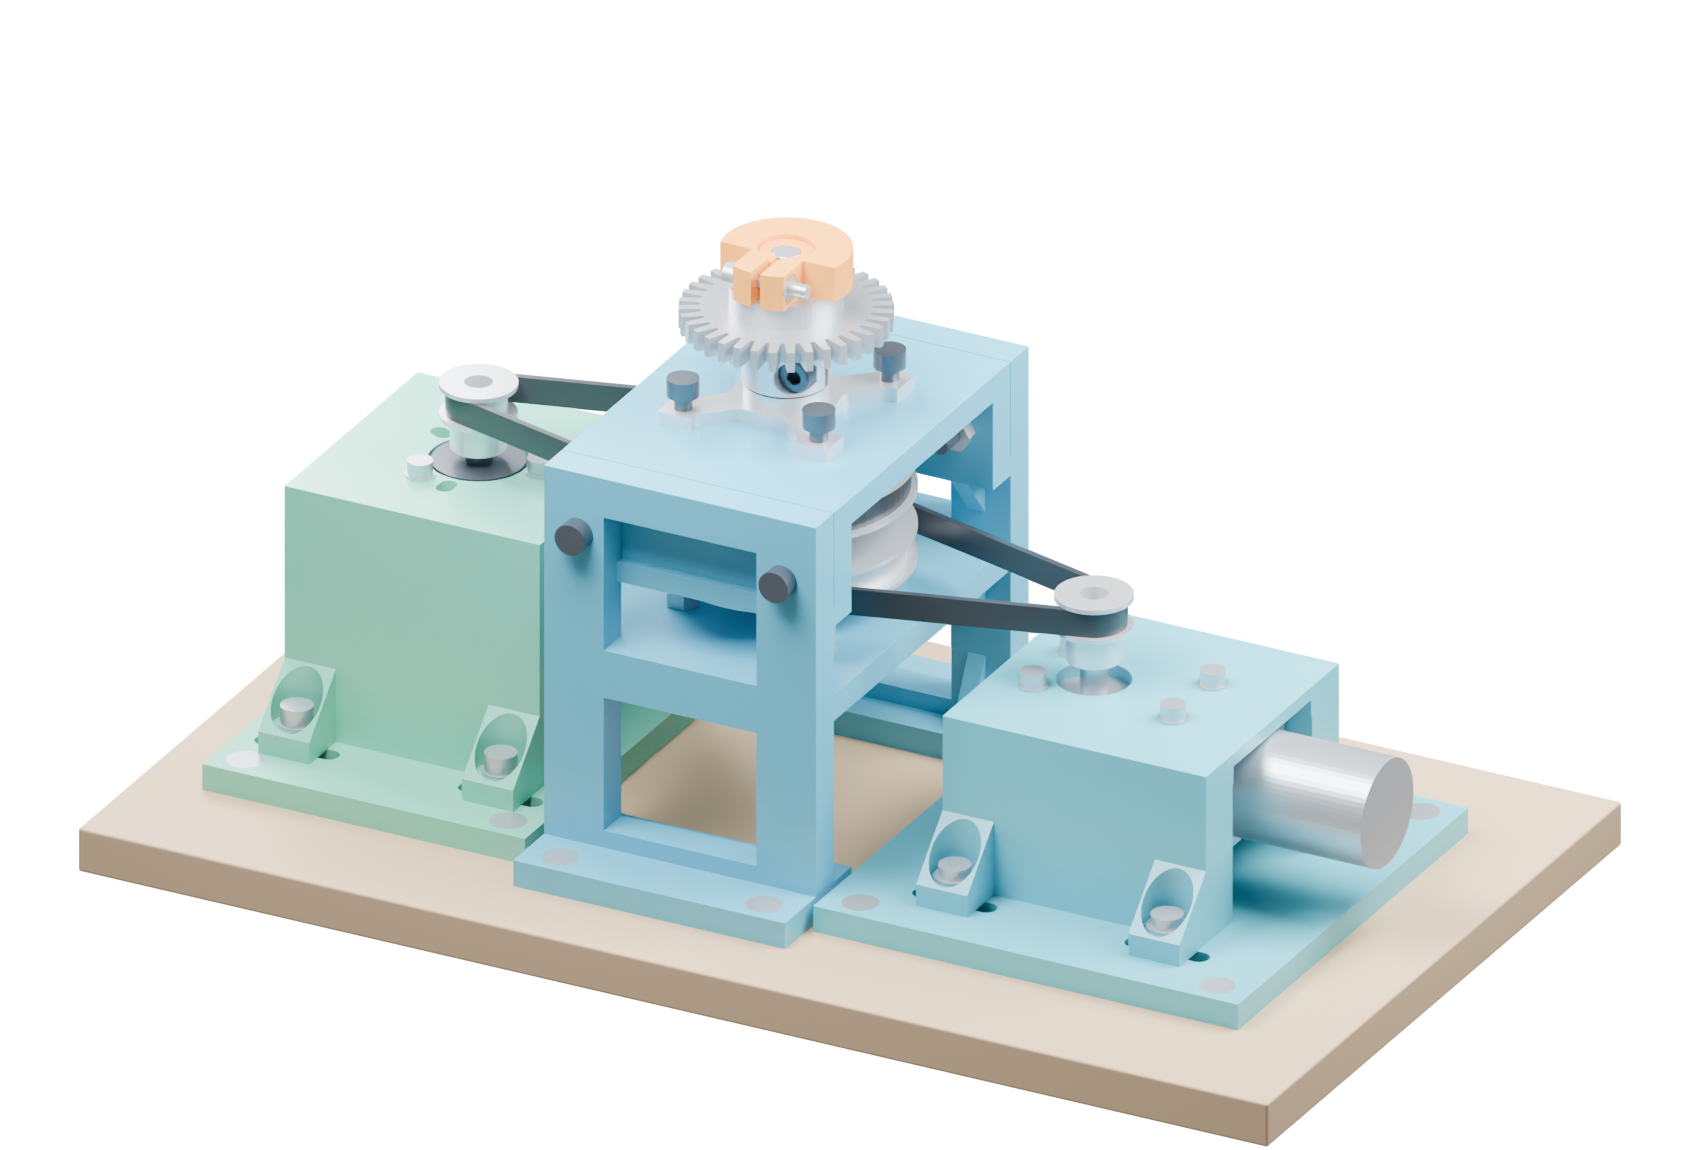
\includegraphics[height=2.7cm,trim=150 120 150 150,clip]{figures/rig_cad.png}
  \caption{LISA optical layout (left) and turntable (right).}
  \label{fig:setup}
\end{figure}

\subsection{Data processing pipeline}

\textbf{Assumptions.} (1) Damage scatters some light into reflection angles a healthy tooth does not reach. (2) That scattering does not shift the peak much. Earlier single-dent simulations support both: the peak moved only $0.007^\circ$ while light moved from the centre to the outer angles.



\textbf{Pipeline.} Each camera image is converted back to reflection angle with the lens mapping, and the light is summed into $2^\circ$ bins over $\pm40^\circ$ around the lens axis in both directions ($40\times40=1{,}600$ numbers). Each frame is divided by its total light, so laser brightness does not matter, square-rooted, so the faint scattered light doesn't get overshadowed by the bright peak, and averaged with the next frame to reduce random noise. Principal component analysis (PCA) fitted on healthy frames reduces each frame to 5 numbers, and the score is the mean distance to the 3 nearest healthy frames ($k$-nearest neighbours, KNN), an idea taken from PatchCore~\cite{roth2022}. A tooth is flagged when any of its frames scores above a cutoff, chosen by F1 on validation data and applied unchanged to the test data. Settings were chosen on validation data only (Section~\ref{sec:results}).

\section{Simulation and data}

We render the setup in Mitsuba~3~\cite{mitsuba3} on the GPU: a 44\,mm, 35-tooth model of the physical gear with machining marks, a rough steel surface (GGX~\cite{walter2007}, $\alpha=0.05$), an ideal 50\,mm collector, and about 4.2 million rays per frame, saved as a $512\times512$ image of the 150\,mm screen. Damage is a spherical cavity with depth equal to its radius on a tooth-top edge, crown, or flank (Fig.~\ref{fig:cavities}), five per damaged gear. Frames are $0.1875^\circ$ apart, matching the encoder trigger. For each cavity we render 16 frames within $\pm1.5^\circ$ of its crossing and label those within $\pm0.4^\circ$ as damaged; two full healthy revolutions (A and B, 1,920 frames each) supply the healthy teeth. Splits hold whole gears: the detector learns from revolution A; validation uses 40 cavities (six random gears at Ø0.10--0.20\,mm and gears 2--3 at Ø0.10\,mm) against 18 teeth of revolution B; and the test, used once, has 30 cavities on gears 1, 4, and 5 at Ø0.10 and Ø0.20\,mm against the other 17 teeth.

\begin{figure}[h]
  \centering
  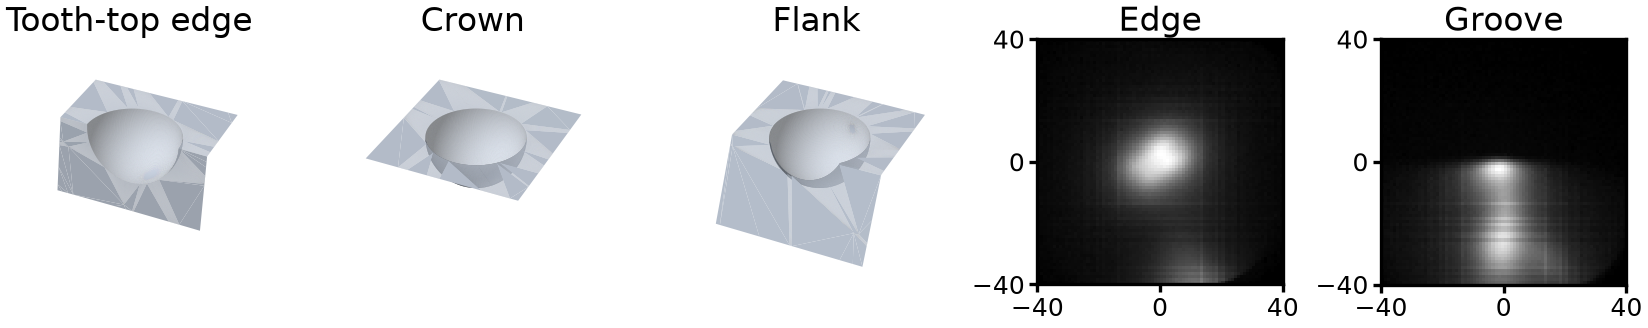
\includegraphics[width=0.9\linewidth]{figures/cavity_types.png}
  \caption{Simulated Ø0.20\,mm cavities (left three) and healthy reflection patterns at a tooth-top edge and the groove, $\pm40^\circ$ in $1^\circ$ bins from $512\times512$ screen images (right two).}
  \label{fig:cavities}
\end{figure}

\section{Results}
\label{sec:results}

\textbf{Choosing the setup on validation data.} Table~\ref{tab:validation} follows the choices in order, each with its F1 cutoff. With 20 PCA numbers, 6 cavities were missed; 5 numbers caught all 40 but flagged 4 of 18 healthy teeth. Requiring 2 frames in a row removed those false alarms but missed 3 cavities, and 3 in a row missed 8. Averaging the angular distributions of neighbouring frames before scoring kept both low: 1 missed cavity and no flagged teeth. Bins of $1^\circ$ and $0.5^\circ$ gave the same counts as $2^\circ$.

\begin{table}[H]
  \centering
  \caption{Validation results for 40 cavities and 18 healthy teeth, with square root, $k=3$, and $2^\circ$ bins.}
  \label{tab:validation}
  \small
  \begin{tabular}{lcccc}
    \toprule
    Setting & TP & FN & FP & TN \\
    \midrule
    PCA 20, single frame & 34 & 6 & 0 & 18 \\
    PCA 5, single frame & 40 & 0 & 4 & 14 \\
    PCA 5, 2 in a row & 37 & 3 & 0 & 18 \\
    PCA 5, 3 in a row & 32 & 8 & 2 & 16 \\
    PCA 5, scores averaged & 40 & 0 & 3 & 15 \\
    \textbf{PCA 5, frames averaged} & \textbf{39} & \textbf{1} & \textbf{0} & \textbf{18} \\
    \bottomrule
  \end{tabular}
\end{table}

\textbf{Test.} There is no physical baseline yet, so PatchCore~\cite{roth2022}, an image-based anomaly detector run on earlier renders of the same test gears, serves as a temporary baseline; its false alarms are counted on the same 17 healthy teeth of its own healthy render. With the chosen setup and its frozen cutoff, our detector missed 4 of 30 test cavities, all Ø0.10\,mm (G1\_D2, G5\_D1, G1\_D5, G5\_D5), and flagged healthy teeth 18, 31, and 34 (Table~\ref{tab:results}). By size, it caught 15/15 Ø0.20\,mm [80--100\%] and 11/15 Ø0.10\,mm [48--89\%] cavities, against 14/15 [70--99\%] and 6/15 [20--64\%] for PatchCore, and flagged 3/17 healthy teeth [6--41\%] against 14/17 [59--94\%]; brackets give 95\% Wilson intervals, the range where the true rate plausibly lies given the small counts. By type, it caught all 6 crown, 16 of 18 edge, and 4 of 6 flank cavities.

\begin{table}[H]
  \centering
  \caption{Test results for 30 cavities and 17 healthy teeth.}
  \label{tab:results}
  \small
  \begin{tabular}{lcccc}
    \toprule
    & TP & FN & FP & TN \\
    \midrule
    Our detector & 26 & 4 & 3 & 14 \\
    PatchCore & 20 & 10 & 14 & 3 \\
    \bottomrule
  \end{tabular}
\end{table}

\textbf{Failed attempts.} Stronger brightness compression (gamma 0.25, log), more PCA numbers (50--100), $k=10$, and scoring by the PCA leftover all separated cavities from healthy teeth less well than the chosen setup.

\section{Conclusion}

In simulation, the detector finds Ø0.20\,mm cavities reliably and Ø0.10\,mm cavities about three times in four, and it flags far fewer healthy teeth than PatchCore on the same test gears (3 against 14 of 17, with non-overlapping intervals). The misses mark the current limit: a missed Ø0.10\,mm cavity changes the angular distribution by only about one-fifth of the render noise, while every validation cavity of Ø0.14\,mm or more was caught.

These results have limits that set the next steps. Healthy revolutions A and B differ only in render noise, so real teeth will match the memory less closely and the false alarms here are optimistic. With 30 test cavities and 17 healthy test teeth the intervals are wide, and the F1 cutoff can move with which cavities and teeth the validation set holds. In simulation, we will therefore plot detection against cavity diameter to locate the limit, render more healthy revolutions to measure false alarms on more teeth, and test a healthy reference built from neighbouring teeth aligned by cross-correlation.

The largest limit is that all evidence is simulated. Next, we will finish building the turntable and collect physical scans by November 20, compare them with the simulation and mix real and simulated data at different ratios to test the thesis by December 2, and complete the final report by December 9. If the build runs late, we will finish the simulation study and check a few real teeth.

\paragraph{Class-survey draft.} \textbf{Case summary.} A laser check for gear-tooth impact damage found all 15 Ø0.20\,mm and 11 of 15 Ø0.10\,mm simulated cavities with 3 of 17 healthy teeth flagged; real scans will test whether simulated damage helps. \textbf{Matrix entry.} Domain, AI role, evidence, difficult condition, and conclusion are as above. Current process: manual inspection with a magnifying glass and rod. Domain requirement: detection judged by probability of detection against defect size, including the size detected with 90\% probability at 95\% confidence~\cite{astm2862}. Response after a change: re-record the healthy memory, recheck the cutoff, and inspect uncertain teeth manually. Reviewer: inspection technician. Open question: does simulated damage help when real damaged examples are few?

\paragraph{Contributions.} Haoxuan Yang built the simulation, is building the physical setup, ran the experiments, and wrote this report. \textbf{Code and project record:} \url{https://github.com/hyang025/synthetic-gear-defect-detection}. \textbf{Generative AI disclosure:} The earlier simulation, PatchCore, and turntable CAD code was written with OpenAI Codex. For this milestone, Claude Code wrote the render, detector, and figure scripts following my method and decisions, suggested choices I approved (square-root scaling, frame averaging, Wilson intervals), and drafted the report text from my direction. I reviewed the results and am responsible for the report.

\small
\begin{thebibliography}{9}
\bibitem{mitsuba3} W.~Jakob, S.~Speierer, N.~Roussel, M.~Nimier-David, D.~Vicini, T.~Zeltner, B.~Nicolet, M.~Crespo, V.~Leroy, and Z.~Zhang. Mitsuba 3 renderer, 2022. \url{https://mitsuba-renderer.org}
\bibitem{walter2007} B.~Walter, S.~R.~Marschner, H.~Li, and K.~E.~Torrance. Microfacet models for refraction through rough surfaces. In \emph{Eurographics Symposium on Rendering}, 2007.
\bibitem{roth2022} K.~Roth, L.~Pemula, J.~Zepeda, B.~Sch\"olkopf, T.~Brox, and P.~Gehler. Towards total recall in industrial anomaly detection. In \emph{CVPR}, 2022.
\bibitem{fulir2023} J.~Fulir, L.~Bosnar, H.~Hagen, and P.~Gospodneti\'c. Synthetic data for defect segmentation on complex metal surfaces. In \emph{CVPR Workshops}, 2023.
\bibitem{astm2862} ASTM International. Standard practice for probability of detection analysis for hit/miss data. ASTM E2862-23, 2023. \url{https://doi.org/10.1520/E2862-23}
\end{thebibliography}

\end{document}
